\chapter{Grundlagen}
\label{grundlagen}

Das folgende Kapitel erläutert die Grundlagen und Notationen, die zum weiteren Verständnis der Arbeit benötigt werden.
Zunächst werden in Unterkapitel~\ref{mathematische_notationen} die grundlegenden Notationen zu Mengen, Vektoren, Matrizen und Tensoren definiert, die im weiteren Verlauf verwendet werden.
Daraufhin folgt in Unterkapitel~\ref{graphentheorie} eine kurze Einführung in das Gebiet der Graphentheorie.
Abschließend führt das Unterkapitel~\ref{convolutional_neural_networks} in das Gebiet der neuronalen Netze und insbesondere der Convolutional Neural Networks ein, auf denen diese Arbeit aufbaut.
Für einen umfassenderen Blick in das Gebiet des \emph{Deep Learnings}, den diese Arbeit nicht leisten kann, sei auf \citeauthor{Nielsen}~\cite{Nielsen} verwiesen.

\section{Mathematische Notationen}
\label{mathematische_notationen}

% Tensor, was bedeutet z.B. $\gls{W}_i$

% Diagonalmatrix

\section{Spektrale Graphentheorie}
\label{spektrale_graphentheorie}

Es gibt 2 große Quellen hier:
\begin{itemize}
  \item Spectral Graph Theory by Chung
  \item Discrete Laplace-Beltrami Operator
\end{itemize}
+ 5 zum Lernen:
\begin{itemize}
  \item Semi Supervised Classification
  \item Fast Localized Spectral Filterung
  \item Wavelets on Graphs via Spectral Graph Theory
  \item The Emerging Field of Signal Processing on Graphs
  \item How powerful are Graph Convolutions? (Review)
\end{itemize}

\subsection{Eigenwerte und Eigenvektoren reell symmetrischer Matrizen}
\label{eigenwerte_symmetrischer_matrizen}

\todo{intro}

$\ma{M} \in \gls{R}^{N \times N}$.
$\gls{eiv} \in \gls{R}^{N}$, $\gls{eiv} \neq \mathbf{0}$.
$\gls{lambda} \in \gls{R}$.
\emph{Eigenwertproblem} $\ma{M}\gls{eiv} = \gls{lambda}\gls{eiv}$.
Zu einem \emph{Eigenwert} $\gls{lambda}$ gibt es unendlich viele (skalierte) \emph{Eigenvektoren} \gls{eiv}.
Wir definieren den Eigenvektor \gls{eiv} eines Eigenwertes \gls{lambda} daher eindeutig über die Bedingung $\left\|\gls{eiv}\right\|_2 = 1$.
Sei \ma{M} weiterhin symmetrisch, \dhe{} $\ma{M} = \ma{M}^{\top}$.
Dann gilt für zwei unterschiedliche Eigenvektoren $\gls{eiv}_1$ und $\gls{eiv}_2$, dass $\gls{eiv}_1 \gls{ortho} \gls{eiv}_2$.
Weiterhin hat \ma{M} genau $N$ reelle Eigenwerte mit ${\left\{\gls{lambda}_i\right\}}_{i=1}^N$.

Wir definieren zu \ma{M} die orthogonale \emph{Eigenvektormatrix} $\gls{Eiv} = \left[\gls{eiv}_1, \ldots, \gls{eiv}_n\right] \in \gls{R}^{N \times N}$, wobei $\gls{Eiv}\gls{Eiv}^{\top}=\gls{I}$, und dessen korrespondierende Eigenwertdiagonalmatrix $\gls{Lambda} = \gls{diag}\left(\left[\gls{lambda}_1, \ldots, \gls{lambda}_N\right]\right)$, \dhe{} $\gls{Lambda}_{ii} = \gls{lambda}_i$.
Dann gilt $\ma{M}\gls{Eiv} = \gls{Eiv}\gls{Lambda}$ und insbesondere ist \ma{M} diagonalisierbar über
\begin{equation}
  \ma{M} = \ma{M}\gls{Eiv}\gls{Eiv}^{\top} = \gls{Eiv}\gls{Lambda}\gls{Eiv}^{\top}.
\end{equation}

Weiterhin gilt für die $k$te Potenz von $\ma{M}$, $k \in \gls{N}$,
\begin{equation}
  \ma{M}^k = {\left(\gls{Eiv}\gls{Lambda}\gls{Eiv}^{\top}\right)}^k = \gls{Eiv}\gls{Lambda}^k\gls{Eiv}^{\top}.
\end{equation}

Dieser Zusammenhang lässt sich verdeutlichen, wenn man die Potenz ausschreibt:
\begin{equation*}
  {\left(\gls{Eiv}\gls{Lambda}\gls{Eiv}^{\top}\right)}^k = \gls{Eiv}\gls{Lambda}\gls{Eiv}^{\top}\gls{Eiv}\gls{Lambda}\gls{Eiv}^{\top}\prod^{k-2}_{i=1} \gls{Eiv}\gls{Lambda}\gls{Eiv}^{\top} = \gls{Eiv}\gls{Lambda}^2\gls{Eiv}^{\top} \prod^{k-2}_{i=1} \gls{Eiv}\gls{Lambda}\gls{Eiv}^{\top} = \gls{Eiv}\gls{Lambda}^k \gls{Eiv}^{\top}.
\end{equation*}

Falls \ma{M} weiterhin \emph{schwach diagonaldominant} ist, \dhe{}
\begin{equation}
  \sum_{\substack{j=1\\j \neq i}}^N \left|\ma{M}_{ij}\right| \leq \left|\ma{M}\right|_{ii},
  \label{eq:schwach_diagonaldominant}
\end{equation}
und $\ma{M}_{ii} \geq 0$ für alle $i \in \left\{1, \ldots, N\right\}$, ist \ma{M} \emph{positiv semidefinit}, \dhe{} $\ve{x}^{\top}\ma{M}\ve{x} \geq 0$ für alle $\ve{x} \in \gls{R}^{N}$.
Eigenwerte symmetrischer positiv semidefiniter Matrizen $\lambda_i \in \gls{R+}$ sind positiv reell und es lässt sich folglich auf diesen eine Ordnung definieren mit $0 \leq \gls{lambda}_1 \leq \cdots \leq \gls{lambda}_N \coloneqq \gls{lambdamax}$.

\todo{quelle}

\subsection{Laplace-Matrix}
\label{laplace_matrix}

Our eigenvalues relate well to other graph invariants for general graphs in a way that other definitions (such as the eigenvalues of adjacency matrices) often fail to do.
The advantages of this definition are perhaps due to the fact that it is consistent with the eigenvalues in spectral geometry and in stochastic processes.
Many results which were only known for regular graphs can be generalized to all graphs~\cite{Chung}.

\todo{intro}

Für einen schleifenlosen, ungerichteteten, gewichtet oder ungewichteten Graphen \gls{G} und dessen Adjazenzmatrix \gls{A} mit Gradmatrix \gls{D} ist die \emph{kombinatorische Laplace-Matrix} \gls{L} definiert als $\gls{L} = \gls{D} - \gls{A}$~\cite{Chung}.
Die \emph{normalisierte Laplace-Matrix} \gls{Lnorm} ist definiert als $\gls{Lnorm} = \gls{D}^{-\frac{1}{2}} \gls{L} \gls{D}^{-\frac{1}{2}}$ mit der Konvention, dass $\gls{D}^{-\frac{1}{2}}_{ii} = 0$ für isolierte Knoten $\gls{v}_i \in \gls{V}$ in \gls{G}, \dhe{} $\gls{D}_{ii} = 0$~\cite{Chung}.
Daraus ergibt sich die elementweise Definition
\begin{equation*}
  \gls{Lnorm}_{ij} = \begin{cases}
  1, & \text{wenn }i = j,\\
    -\frac{\gls{w}\left(\gls{v}_i, \gls{v}_j\right)}{\sqrt{\gls{d}\left(\gls{v}_i\right)\gls{d}\left(\gls{v}_j\right)}}, & \text{wenn }\gls{v}_i \gls{adj} \gls{v}_j,\\
  0, & \text{sonst.}
\end{cases}
\end{equation*}
Für verbundene Graphen kann \gls{Lnorm} vereinfacht werden zu $\gls{Lnorm} = \gls{I} - \gls{D}^{-\frac{1}{2}} \gls{A} \gls{D}^{-\frac{1}{2}}$~\cite{Chung}.
Jeder Eintrag auf der Diagonalen der normalisierten Laplace-Matrix ist folglich Eins.
\gls{Lnorm} ist damit normalisiert auf den (gewichteten) Grad zweier adjazenter Knoten $\gls{v}_i$ und $\gls{v}_j$.
Es ist anzumerken, dass \gls{L} und insbesondere \gls{Lnorm} symmetrisch sind, wohingegen eine Normalisierung der Form $\gls{D}^{-1}\gls{L}$ dies in der Regel nicht wäre~\cite{Reuter}.

\gls{L} und \gls{Lnorm} sind keine ähnlichen Matrizen.
Insbesondere sind ihre Eigenvektoren unterschiedlich.
Die Nutzung von \gls{L} oder \gls{Lnorm} ist damit abhängig von dem Problem, welches man betrachtet~\cite{Hammond}.
Wir schreiben \gls{Lboth} wenn die Wahl der Laplace-Matrix, ob \gls{L} oder \gls{Lnorm}, für die weitere Berechnung zwar fest, aber irrelevant ist.

\paragraph{Interpretation}
\label{laplace_interpretation}

\todo{kurz laplace beltrami}

Sei $\ve{f} \in \gls{R}^N$ eine Funktion \bzw{} ein Signal auf den Knoten eines Graphen \gls{G}.
Dann kann für die kombinatorische Laplace-Matrix \gls{L} verifiziert werden, dass \gls{L} die Gleichung
\begin{equation*}
  {\left(\gls{L}\ve{f}\right)}_i = \sum_{i \gls{adj} j} \gls{w}\left(\gls{v}_i, \gls{v}_j\right) \left(\ve{f}_i - \ve{f}_j\right)
\end{equation*}
erfüllt~\cite{Hammond}.
Sei $\gls{G}$ nun ein Graph, der aus einem (unendlichen) zweidimensionalen regulärem Gitter entstanden ist, \dhe{} jeder Knoten $\gls{v}_i$ besitzt genau $4$ Nachbarn mit gleichen Kantengewichten $\frac{1}{\delta^2}$, wobei $\delta \in \gls{R}$ beliebige Konstante.
Zur einfacheren Veranschaulichung benutzen wir dabei für die Signalstärke $\ve{f}_i$ eines Knoten $v_i$ an Position $\left(x, y\right)$ die Indexnotation $\ve{f}_{x,y}$.
Dann beschreibt
\begin{equation*}
  {\left(\gls{L}\ve{f}\right)}_{x,y} = \frac{4\ve{f}_{x,y} - \ve{f}_{x+1,y} - \ve{f}_{x-1,y} - \ve{f}_{x,y+1} - \ve{f}_{x,y-1}}{h^2}
\end{equation*}
die \emph{5-Punkte-Stern} Approximation $-\nabla^2 f$ (bei umgekehrtem Vorzeichen) definiert auf den Punkten $\left\{\left(x,y\right), \left(x+\delta,y\right), \left(x-\delta,y\right), \left(x,\delta+h\right),\left(x,y-\delta\right)\right\}$~\cite{Hammond}.\todo{grafik}
Ähnlich zu einem regulären Gitter lässt sich ein Graph \gls{G} auch über beliebig viele Abtastpunkte einer differenzierbaren Mannigfaltigkeit konstruieren.
Es zeigt sich, dass mit steigender Abtastdichte und geeigneter Wahl der Kantengewichte die normalisierte Laplace-Matrix \gls{Lnorm} zu dem kontinuierlichem Laplace-Beltrami Operator konvergiert~\cite{Hammond}.
Damit kann $\gls{Lnorm}$ als die diskrete Analogie des $\nabla^2$ Operators auf Graphen verstanden werden.
Der Laplace-Beltrami Operator misst dabei, in wie weit sich eine Funktion $f$ an einem Punkt $x$ von dem Durchschnitt aller Funktionspunkte um einen kleinen Bereich um $x$ unterscheidet.
Die Laplace-Matrix operiert dabei völlig analog, in dem sie misst, wie sehr sich eine (diskrete) Funktion um einen Knoten im Vergleich zu seinen Nachbarknoten unterscheidet.

Eigenwerte und Eigenvektoren von \gls{Lboth} helfen uns dabei, die lineare Transformation einer Funktion \ve{f} (mehrfach) angewendet auf \gls{Lboth} besser zu verstehen.
Wir können dafür \ve{f} als Linearkombination der Eigenbasis $\sum_i c_i \gls{eiv}_i$ schreiben und erhalten
\begin{equation*}
  \gls{Lboth}^k \ve{f} = \sum_i c_i \gls{Lboth}^k \gls{eiv}_i = \sum_i c_i \gls{lambda}_i^k \gls{eiv}_i.
\end{equation*}
Somit können Eigenschaften von \gls{Lboth} und damit des Graphen selber durch dessen Eigenwerte und Eigenvektoren beschrieben werden.

\paragraph{Eigenschaften}
\label{laplace_eigenschaften}

$\gls{Lboth} \in \gls{R}^{N \times N}$ ist eine reell symmetrisch, positiv semidefinite Matrix~\cite{Chung}.
Folglich besitzt \gls{Lboth} nach Kapitel~\ref{eigenwerte_symmetrischer_matrizen} genau $N$ positiv reelle Eigenwerte ${\left\{\gls{lambda}_i\right\}}_{i=1}^N$ mit Ordnung $0 \leq \gls{lambda}_1 \leq \cdots \leq \gls{lambda}_N$ und $N$ korrespondierende orthogonale Eigenvektoren ${\left\{\gls{eiv}_i\right\}}_{i=1}^N$.

Die kombinatorische Laplace-Matrix $\gls{L}$ ist nach~\eqref{eq:schwach_diagonaldominant} weiterhin schwach diagonaldominant.
Insbesondere summiert sich jede Reihen- und Spaltensumme von \gls{L} zu Null auf, \dhe{} $\sum_{j=1}^N \gls{L}_{ij} = \sum_{j=1}^N \gls{L}_{ji} = 0$.
Daraus folgt unmittelbar, dass $\gls{lambda}_1 = 0$, da $\gls{eiv}_1 = \frac{1}{\sqrt{N}}{\left[1, \ldots, 1\right]}^{\top} \in \gls{R}^N$ Eigenvektor von \gls{L} mit $\gls{L}\gls{eiv}_1 = \ve{0}$.
\gls{Lnorm} hingegen ist nicht zwingend schwach diagonaldominant.
Es lässt sich jedoch zeigen, dass auch für \gls{Lnorm} gilt, dass $\gls{lambda}_1 = 0$~\cite{Chung}.

Eine der interessantesten Eigenschaften eines Graphs ist dessen Konnektivität.
Die Laplace-Matrix \gls{Lboth} \bzw{} dessen Eigenwerte stellen ein geeignetes Mittel zur Untersuchung dieser Eigenschaft dar.
So gilt \zB{} für einen verbundenen Graphen \gls{G}, dass $\gls{lambda}_2 > 0$.
Falls $\gls{lambda}_i = 0$ und $\gls{lambda}_{i+1} \neq 0$, dann besitzt $\gls{G}$ genau $i$ verbundene Komponenten~\cite{Chung}.
Damit ist die Anzahl der Null-Eigenwerte äquivalent zu der Anzahl an Komponenten, die ein Graph besitzt.
Für \gls{Lnorm} lässt sich weiterhin zeigen, dass $\gls{lambdamax} \leq 2$ eine obere Schranke ihrer Eigenwerte ist~\cite{Chung}.

Aus der Laplace-Matrix können ebenso Rückschlüsse über die kürzeste Pfadlänge zweier Knoten gewonnen werden.
So gilt für $\gls{Lboth}^{k}$ mit $k \in \gls{N}$, dass $\gls{Lboth}^k_{ij} = 0$ genau dann, wenn $\gls{s}\left(v_i, v_j\right) > k$~\cite{Hammond}.
Damit beschreibt $\gls{Lboth}^k_i$ bildlich gesprochen die Menge an Knoten, die maximal $k$ Kanten von $i$ entfernt liegen.

\section{Convolutional Neural Networks}
\label{convolutional_neural_networks}

Neuronale Netze \bzw{} Deep-Learning gehören zu den derzeit besten und beliebtesten Lösungen zu Problemen der Bild- oder Spracherkennung~\cite{Nielsen}.
Dabei lernt \bzw{} approximiert das Netz durch eine Anpassung ihrer Parameter über einer Menge an Trainingsbeispielen eine stetige Funktion, sodass die Trainingsbeispiele auf ihre gewünschte Ausgabe abbilden und auch für unbekannte Eingaben zuverlässige Vorhersagen getroffen werden können.
Neuronale Netze sind daher größtenteils in dem Bereich des \emph{überwachten maschinellen Lernens} anzuordnen.
Ein Netz, welches lediglich die Trainingsmenge lernt und dessen Parameter unbekannte Eingaben nicht generalisieren können, wird als ein \emph{überangepasstes} (\engl{} \emph{overfitted}) Netz bezeichnet~\cite{Nielsen}.

Ein \emph{neuronales Netz} besteht aus einer beliebigen Anzahl miteinander verbundener \emph{Neuronen}.
Neuronen sind üblicherweise mit anderen Neuronen in sequentiellen \emph{Schichten} \bzw{} \emph{Ebenen} angeordnet.
Die erste Schicht eines neuronalen Netzes wird als \emph{Eingabe}- und die letzte Schicht als  \emph{Ausgabeschicht} bezeichnet.
Schichten zwischen Ein- und Ausgabe heißen \emph{versteckt} (\engl{} \emph{hidden}).
Als \emph{Deep-Learning} wird ein Netz mit mindestens zwei versteckten Schichten verstanden.
Die einfachste Form eines neuronalen Netzes ist das \emph{Feedforward}-Netz, bei der jedes Neuron einer Schicht mit allen Neuronen der darauffolgenden Schicht verbunden ist.
Die Schichten eines Feedforward-Netzes werden deshalb auch als \emph{vollverbunden} (\engl{} \emph{fully-connected}) betitelt.
Abbildung~\ref{fig:feedforward} zeigt ein Beispiel eines solchen Netzes mit drei Schichten.
\begin{figure}[t]
\centering
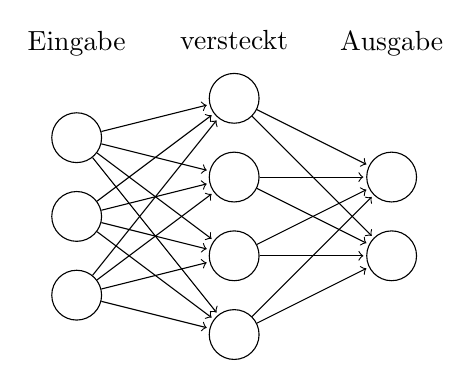
\begin{tikzpicture}
  \tikzstyle{node}=[circle,draw, minimum width=18pt, inner sep=0pt, fill=white]
  \tikzstyle{edge}=[->, shorten >= 1pt]

  \node[rectangle, inner sep=0pt] at (-2, 2.2) {Eingabe};
  \node[rectangle, inner sep=1pt] at (0,  2.24) {versteckt};
  \node[rectangle, inner sep=0pt] at (2,  2.2) {Ausgabe};

  \node[node] (a1) at (-2, -1) {};
  \node[node] (a2) at (-2, 0)  {};
  \node[node] (a3) at (-2, 1)  {};

  \node[node] (b1) at (0, -1.5) {};
  \node[node] (b2) at (0, -0.5) {};
  \node[node] (b3) at (0, 0.5)  {};
  \node[node] (b4) at (0, 1.5)  {};

  \node[node] (c1) at (2, -0.5) {};
  \node[node] (c2) at (2, 0.5)  {};

  \path[edge] (a1) edge (b1);
  \path[edge] (a1) edge (b2);
  \path[edge] (a1) edge (b3);
  \path[edge] (a1) edge (b4);
  \path[edge] (a2) edge (b1);
  \path[edge] (a2) edge (b2);
  \path[edge] (a2) edge (b3);
  \path[edge] (a2) edge (b4);
  \path[edge] (a3) edge (b1);
  \path[edge] (a3) edge (b2);
  \path[edge] (a3) edge (b3);
  \path[edge] (a3) edge (b4);
  \path[edge] (b1) edge (c1);
  \path[edge] (b1) edge (c2);
  \path[edge] (b2) edge (c1);
  \path[edge] (b2) edge (c2);
  \path[edge] (b3) edge (c1);
  \path[edge] (b3) edge (c2);
  \path[edge] (b4) edge (c1);
  \path[edge] (b4) edge (c2);
\end{tikzpicture}
\caption[Feedforward-Netz]{Beispiel eines Feedforward-Netzes mit drei vollverbundenen Schichten von einer Eingabe mit drei Neuronen zu einer Ausgabe mit zwei Neuronen und einer dazwischenliegenden versteckten Schicht.}
\label{fig:feedforward}
\end{figure}

Andere Netzvarianten erlauben \zB{} Schleifen, Rückwärtskanten oder das Überspringen einer Schicht~\cite{Nielsen}.

Ein Neuron besitzt genau einen reellen Wert, der sich aus den Neuronen der vorherigen Schicht erschließt.
Die $t$-te Neuronenschicht lässt sich folglich als ein Vektor $\ve{x}^{\left(t\right)} \in \gls{R}^{N^{\left(t\right)}}$ auffassen, wobei $N^{\left(t\right)} \in \gls{N}$ die Anzahl der Neuronen in der $t$-ten Schicht beschreibt.
Zu jeder Kante existiert zusätzlich ein Gewicht, welches den Anteil des Neurons zu dessen verbundenen Neuron angibt.
Damit lassen sich die Neuronenwerte der $\left(t+1\right)$-ten Schicht über
\begin{equation*}
  \ve{x}^{\left(t+1\right)} \coloneqq \gls{W}^{\left(t+1\right)}\ve{x}^{\left(t\right)}
\end{equation*}
definieren, wobei $\gls{W}^{\left(t+1\right)} \in \gls{R}^{N^{\left(t+1\right)} \times N^{\left(t\right)}}$ eine \emph{Gewichtsmatrix} der Kanten beschreibt, sodass $\gls{W}^{\left(t+1\right)}_{ji} \in \gls{R}$ das Gewicht der Kante des $i$-ten Neurons in der $t$-ten Schicht zu dem $j$-ten Neuron der $\left(t+1\right)$-ten Schicht angibt.
Zusätzlich zu den Gewichten existert zu jedem Neuron in der $t$-ten Schicht außer der Eingabeschicht ein \emph{Bias} $\gls{b}^{\left(t\right)} \in \gls{R}^{N^{\left(t\right)}}$.
Mit einer elementweisen Anwendung einer nicht-linearen \emph{Aktivierungsfunktion} $\gls{act} \colon \gls{R} \to \gls{R}$ ergibt sich damit die finale Version der Neuronenwerte der $\left(t+1\right)$-ten Schicht als
\begin{equation*}
  \ve{x}^{\left(t+1\right)} \coloneqq \gls{act} \left(\gls{W}^{\left(t+1\right)}\ve{x}^{\left(t\right)} + \gls{b}^{\left(t+1\right)} \right).
\end{equation*}
Als Aktivierungsfunktion kommt dabei \bspw{} die nicht-lineare \emph{Sigmoidfunktion} $\mathrm{sig}\left(z\right) \coloneqq 1 / \left(1 + \exp\left(-z\right)\right)$ oder die \emph{Rectified Linear Unit (ReLU)}-Funktion $\gls{relu}\left(z\right) \coloneqq \max \left(z, 0\right)$ zum Einsatz~\cite{Nielsen}.
Die Menge der Gewichte $\mathcal{W} \coloneqq {\left\{\gls{W}^{\left(t\right)}\right\}}_{t=2}^T$ sowie die Menge der Biaswerte $\mathcal{B} \coloneqq {\left\{\gls{b}^{\left(t\right)}\right\}}_{t=2}^T$ für $T \in \gls{N}$ viele Schichten werden die \emph{Parameter} des Netzes genannt, über dessen Anpassung das Netz trainiert wird.
Diese Werte werden dabei sequentiell über eine kleine Eingabemenge $\mathcal{X} \coloneqq {\left\{\ve{x}_n \right\}}_{n=1}^N$ so angepasst, dass eine \emph{Kostenfunktion} minimiert wird.
Die \emph{quadratische Kostenfunktion}




\begin{equation*}
  \mathrm{quadratische kostenfunktion}
  \label{eq:quadratische_kostenfunktion}
\end{equation*}





% Epoche
% Learning-Rate
% Loss-Function

% Receptive-Field
% Merkmalskarten oder Featuremap
% Backpropagation quelle
% Stride, Filtergröße
% Stride Slice Pooling
% genereller Faltungsoperator?
\gls{conv2d}
\gls{CNN}

% What we'd like is an algorithm which lets us find weights and biases so that the output from the network approximates y(x)y(x) for all training inputs xx. To quantify how well we're achieving this goal we define a cost function*

% Üblicherweise wird \gls{learning} so gewählt, dass nicht zu langsam gelernt wird, aber dennoch eine gute Approximation erreicht wird.

